\cotefile{149}

\scanpage{103}
\mspage{51}
On a évidemment $\mathrm{a)}\Rightarrow\mathrm{b)}\Rightarrow\mathrm{c)}\unsure{=|\Rightarrow}\mathrm{d)}$,
et $d\Rightarrow a$ devrait être plus ou moins
connu, ou du moins se prouver à
l'aide de choses bien connues. Ces
conditions impliquent e, mais je n'ai
pas d'idée pour le moment comment
voir que e) implique bonne réduction ---
faudrait une compréhension (fut-elle
heuristique) plus approfondie que celle
que j'ai pour le moment.
\margin{Ça vaudrait la peine de regarder une version de ceci où $X_\eta=\hat U_\eta$ a bonne réduction --- mais la multisection $\overline{X_\eta-U_\eta}$ de $X$ sur $S$ n'est pas étale. Le cas du genre $0$ devrait être particulièrement aisé à regarder\ldots}

J'ai donc là un principe général
(que je pourrais à l'occasion formuler
avec la généralité qui lui convient) pour
construire des actions extérieures \inserted{Individuelles}
de groupes $\mathcal E_k$ ($k$ \deleted{ext.} de type fini
de $\mathbb{Q}$) sur des $\pi$ à bouts, qui
\inserted{(sans \unsure{doute|doute\ldots})}
ne soient géométriques, par \deleted{\unsure{des|de}} la
considération de courbes de type $g,\nu$
``se réduisant mal''. Mais je n'arrive
\margin{102}

\scanpage{105}
\mspage{52}
4. \uline{Sections \inserted{d'extensions,} et anneaux de valuation généraux.}

D'abord une révision de notations. Si $X$ est un schéma connexe, je \deleted{\unsure{dé|de}}note \deleted{$\mathcal E_X$}
\[
(1)\qquad \mathcal E_X=\Pi_1(X)
\]
son groupe fond. profini en tant que groupe extérieur, et si $\tilde X$ est un rev. universel profini de $\mathcal E_X$, par
\[
(2)\qquad \mathcal E_X^{(\tilde X)}=\Pi_1(X;\tilde X)=\operatorname{Aut}_X(\tilde X)
\]
son groupe fondamental précisé --- qui est un groupe profini. Si $X=\operatorname{Spec}(A)$, où $A$ est un anneau (le plus souvent un corps) je note $\mathcal E_A$, et $\mathcal E_A^{\tilde A}$ \inserted{$=\mathcal E_X^{\unsure{\tilde X|X}}$} si $\tilde A$ est une $A$-algèbre telle que $\operatorname{Spec}(\tilde A)=\tilde X$ soit un rev. universel de $X$ (ce qui le détermine à isom non unique près). Bien entendu, si $\unsure{\zeta|\xi}$ est un ``point géométrique'' de $X$, on note
\[
(3)\qquad \mathcal E_X^{\unsure{\zeta|\xi}}=\Pi_1(X,\unsure{\zeta|\xi})=\mathcal E_X^{\tilde X(\unsure{\zeta|\xi})},
\]
où $\tilde X(\unsure{\zeta|\xi})$ est le \unsure{rev|rev.} universel de $X$ pointé en $\unsure{\zeta|\xi}$. Le choix
\margin{104}

\scanpage{106}
de $\unsure{\zeta|\xi}$ correspond au choix d'un $x\in X$ et d'une ext. sép. close \deleted{$\bar K$} \inserted{$\Omega$} de $k(x)$ (pas néc. \deleted{\unsure{une}} clôture alg. de $k(x)$) et on note alors aussi $\mathcal E_X^\Omega$ au lieu de $\mathcal E_X^{\unsure{\zeta|\xi}}$ ($\Omega$ sous-entendu en tant qu'extension de $k(x)$, donc avec sa structure de $k(x)$ algèbre). On aura \inserted{un isom \unsure{can|can.}}
\[
(4)\qquad \mathcal E_{\unsure{\alpha|x}}^\Omega\simeq\mathcal E_X^{\overline{k(x)}},
\]
où $\overline{k(x)}$ est la clôture alg. de $k(x)$ dans $\Omega$. Bien sûr, si $X=\operatorname{Spec}(A)$, on notera aussi $\mathcal E_A^\Omega$ --- notation surtout utilisée pour $\mathcal E_K^{\bar K}$, $K$ un corps, $\bar K$ une clôture alg. ou sép. de $K$.

Si $X$ est un $Y$-schéma, \inserted{$Y$ connexe,} on notera
\[
(5)\qquad \mathcal E(f):\mathcal E_X\longrightarrow\mathcal E_Y\qquad\text{où }f:X\longrightarrow Y
\]
($\mathcal E_X$ est un foncteur en $X$
\[
(\text{Sch conn})\longrightarrow\text{grpes ext}
\]
\margin{105}

\scanpage{107}
\mspage{53}

qui se précise par l'hom effectif de groupes profinis
\[
(6)\qquad \mathcal E_X^{\widetilde X}\longrightarrow\mathcal E_Y^{\widetilde Y}
\]
où $\widetilde Y$ est le rev. universel de $Y$ défini par $\widetilde X\longrightarrow Y$ ($\widetilde X$ jouant le rôle du point --- on devrait pouvoir écrire en fait $\mathcal E_Y^{\widetilde X}$, plus gén. $\mathcal E_Y^Z$ chaque fois qu'on a un $Y$-schéma $Z$ $1$-connexe, jouant le rôle de ``foncteur fibre'' pour le topos $B_{\Pi(X)}$ des rev étales de $Y$\ldots)

\deleted{\unsure{que|qui} $\mathcal E_X^{\unsure{\widetilde X|\widetilde\alpha}}$}

On peut dire que
\[
(7)\qquad (X,\widetilde X)\longmapsto\mathcal E_X^{\widetilde X}
\]
est un foncteur, de la catégorie des schémas $0$-connexes $X$ \uline{munis} d'un rev. universel (ou seulement d'un $Z$ $1$-connexe s'envoyant dans $X$) vers celle des groupes profinis. Ceci s'applique en particulier en regardant la \inserted{sous-}cat. des $(X,\unsure{\zeta|\xi})$ munis d'un $p^t$ géom ---

\margin{106}

\scanpage{108}

on a donc
\[
(8)\qquad \mathcal E_X^{\unsure{\zeta|\xi}}\longrightarrow\mathcal E_{\deleted{\unsure{X|Y}}Y}^\eta
\]
si on a un hom de schémas ``géom\textsuperscript{t}.
ponctués'' $(X,\unsure{\zeta|\xi})\longrightarrow(Y,\eta)$. On
notera que \unsure{tte|tt} ponctuation géom.
de $X$ en un $x\in X$ --- i.e. une
ext. sep close $\Omega$ de $k(x)$ ---
définit \inserted{can\textsuperscript{t}} une ponctuation \inserted{géom} aussi \unsure{de}
de $Y$ en $y=f(x)$, \deleted{par} par composition
--- $\Omega$ ``est'' une extension de $k(y)$ puisque
$k(\underset{\inserted{x}}{\unsure{x}})\hookleftarrow k(y)$ --- et l'hom (8)
s'identifie aussi à
\[
(9)\qquad \mathcal E_X^{\overline{k(x)}}\longrightarrow\mathcal E_Y^{\overline{k(y)}},
\]
où $\overline{k(x)}$, $\overline{k(y)}$ sont les clôtures séparables
\uline{dans $\Omega$}.

On posera
\[
(10)\qquad \mathcal E_{X/Y}^{\widetilde X}=\operatorname{Ker}\bigl(\mathcal E_X^{\widetilde X}\longrightarrow\mathcal E_Y^{\widetilde X}=\mathcal E_Y^{\widetilde Y}\bigr)
\]

\margin{107}

\scanpage{109}
\mspage{54}

(C'est un foncteur p.r. au triple $\widetilde X\longrightarrow X\longrightarrow Y$ avec $X,Y$ $0$-\unsure{connexes|connexe}, $\widetilde X$ un rev. universel; plus généralt, si $\deleted{Z}\inserted{T}\longrightarrow X$ avec $\deleted{Z}\inserted{T}$ $1$-connexe, on pose
\[
(11)\qquad \unsure{\mathcal E}_{X/Y}^{\deleted{Z}\inserted{T}}=\operatorname{Ker}\bigl(\mathcal E_X^{\deleted{Z}\inserted{T}}\longrightarrow\mathcal E_Y^{\deleted{Z}\inserted{T}}\bigr)
\]
on a un foncteur en \inserted{le triple} $(\deleted{Z}\inserted{T}\longrightarrow X_{\unsure{0|\bullet}}\longrightarrow Y)$ variable. En particulier: $\mathcal E_{X/Y}^{\unsure{\zeta|\xi}}$, $\unsure{\zeta|\xi}$ un $p^t$ géom. de $X$, $\mathcal E_{X/Y}^{\Omega}$, $\mathcal E_{X/A}^{\widetilde X}$ (si $Y=\operatorname{Spec} A$), $\mathcal E_{B/A}^{\widetilde B}$ $\ldots$

\margin{\uline{NB} $\mathcal E_{X/Y}^T$, pour $T$ variable, $X/Y$ fixé, est défini à isom non unique !) près, et se note $\mathcal E_{X/Y}$ \unsure{simplem\textsuperscript{t}.}}

Un cas intéressant est celui où on dispose d'une ``suite exacte d'homotopie universelle'' \deleted{de} (en dim $1$) pour $X\longrightarrow Y$, alors la donnée (pour $X=Y$ donné) de $T\longrightarrow X$, (avec $T$ $1$-connexe) peut s'interpréter par la donnée du composé

\margin{Car \unsure{où|à} $\mathcal E_X^{\deleted{Z}\inserted{T}}\longrightarrow\mathcal E_Y^{\deleted{Z}\inserted{T}}$ est \unsure{épi|épi.}}
\margin{108}

\scanpage{110}

\[
T\longrightarrow Y
\]
\uline{et} d'un relèvement en $T\longrightarrow X$, ou ce qui revient au $=$, d'une section de $X_T=X\times_YT$ sur $T$. Ceci posé,

\noindent
\begin{minipage}[t]{0.48\linewidth}
\vspace*{\baselineskip}
\diagram{\begin{tikzcd}
X\arrow[d] & X_T\arrow[l]\arrow[d] & \\
Y & T\arrow[l] & T\arrow[ul, "{\unsure{}}"{description,pos=0.18}]\arrow[l,phantom,"=" description]
\end{tikzcd}}
% The question near the diagonal's lower-right end marks the possible second
% arrowhead there. The upper-left head is certain; the short lower-right return
% may be a tail return or a second head. See the whole-diagram audit and doubt.
\end{minipage}\hfill
\begin{minipage}[t]{0.48\linewidth}
on aura un isom can (sous l'hyp. de ``suite exacte d'homotopie'' \deleted{\unsure{)}} faite)
\end{minipage}

\[
(12)\qquad \mathcal E_{X/Y}^T\simeq\Pi_1(X_T;T)\simeq\mathcal E_{X_T}^T
\]
et on aura
\[
(13)\qquad 1\longrightarrow\mathcal E_{X/Y}^T\longrightarrow\mathcal E_X^T\longrightarrow\mathcal E_Y^T\longrightarrow1
\]
(Cette hypothèse sera tjrs satisfaite si $Y=\operatorname{Spec}K$, $K$ un corps, si $X$ est géom. $0$-connexe sur $K$)

Plus généralement, si on a une suite exacte d'homotopie universelle, mais pas néc. avec $\mathcal E_X^T\longrightarrow\mathcal E_Y^T$ surj,

\margin{109}

\scanpage{111}
\mspage{55}

\margin{Sous l'hyp. ``suite exacte d'homo-\newline topie'', mais avec fibres pas néc. \unsure{connexes|conn.}}

on aura une factorisation can. de
$X\longrightarrow Y$ en
\[
(14)\qquad X\longrightarrow Y'\longrightarrow Y
\]
avec $Y'$ étale fini ou pro-étale fini sur $Y$
et $\mathcal E_X'\longrightarrow\mathcal E_{Y'}$ est maintenant épi,
\deleted{\unsure{donc}} cette suite exacte univ. d'homotopie
bien sûr. On aura des iso can
\[
(15)\qquad \mathcal E_{X/Y}^T\xrightarrow{\sim}\mathcal E_{X/Y'}^T
\]
qui peut donc se calculer comme
\[
(16)\qquad \mathcal E_{X\times_{Y'}T}^T\simeq\mathcal E_{X/Y}^T
\]
qu'on peut noter $\mathcal E_{X_T}^T$, mais en
faisant attention que maintenant
$X_T$ désigne non plus $X\times_YT$ (qui
va être disconnexe \inserted{si $Y'\longrightarrow Y$ pas iso}) mais $X\times_YT$.

Bien sur, à iso. can. près on peut
\deleted{\unsure{en|et}} remplacer, pour le calcul de $\mathcal E_{X_T}^T$,
$T$ par $\widetilde Y$ pour ce qui est du $X_T$, et par
$\widetilde X$ pour ce qui est de l'ancrage dans $X_{\widetilde Y}$,

\margin{110}

\scanpage{112}

où $\widetilde X,\widetilde Y$ sont les rev. universels de $X,Y$ déduits de \inserted{$\unsure{T}\longrightarrow X$ et de $T\longrightarrow Y$,} de telle façon que l'on obtient
\[
(17)\qquad \mathcal E_{X/Y}^T\simeq\mathcal E_{X/Y}^{\widetilde X}\simeq\operatorname{Ker}\bigl(\mathcal E_X^{\widetilde X}\longrightarrow\mathcal E_Y^{\widetilde Y}\bigr)
\]
(sans hyp de suite exacte)

et
\[
\begin{aligned}
&\inserted{\mathcal E_{X_{\widetilde Y}}^Z\simeq\mathcal E_{X_{\widetilde Y}}^{\widetilde X}}\\
(18)\qquad \mathcal E_{X/Y}^T\simeq{}&\deleted{\operatorname{Ker}\bigl(\unsure{\mathcal E_{X_{\widetilde Y}}^{\widetilde X}}\unsure{\mathrel{\text{---}}|\longrightarrow}\unsure{\mathcal E_{\widetilde Y}^{\widetilde Y}}\bigr)}
\end{aligned}
\]
dans le cas général.

\diagram{\begin{tikzcd}
X\arrow[d] & X_{\widetilde Y}\arrow[l]\arrow[d] & \widetilde X\arrow[l] & Z\arrow[l]\\
Y'\arrow[d] & \widetilde Y\arrow[l] & & \\
Y & & &
\end{tikzcd}}

Une autre interprétation de $\mathcal E_{X/Y}^T$ s'obtient en prenant $T$ réduit à un $p^t$ géométrique \inserted{$\unsure{\zeta|\xi}_X$}, qui définit donc un $p^t$ géom. $\unsure{\zeta|\xi}_Y$ de $Y$, une fibre géom. $X_{\unsure{\zeta|\xi}_Y}$ de $X$ sur $Y$ en $\unsure{\zeta|\xi}_Y$, $\unsure{\zeta|\xi}_X$ s'interprétant comme un $p^t$ géom. de cette fibre, et on aura
\[
(19)\qquad \mathcal E_{X/Y}^{\unsure{\zeta|\xi}_X}\simeq\mathcal E_{X_{(\unsure{\zeta|\xi}_Y)}}^{\unsure{\zeta|\xi}_X}\simeq\Pi_1(X_{(\unsure{\zeta|\xi}_Y)},\unsure{\zeta|\xi}_X)
\]
--- i.e. $\mathcal E_{X/Y}$ s'interprète comme groupe fondamental des ``fibres géom'' de $X/Y$.

\margin{111}

\scanpage{113}
\mspage{56}

Le lien avec la \deleted{\unsure{definition|définition}}\inserted{\unsure{description|plus ample}} (11) est évidemment que, si $\unsure{\zeta|\xi}_X$ provient d'un $\unsure{p^t|pt}$ géom $\unsure{\zeta|\xi}_T$ de $T$, alors on aura des iso can

\[
\begin{aligned}
(20)\quad &\mathcal E_{X/Y}^{\unsure{\zeta|\xi}_T}\simeq\mathcal E_{X/Y}^T\\[0.5ex]
&\quad\rotatebox{90}{$\simeq$}\\[0.5ex]
&\Pi_1(X_{\unsure{\zeta|\xi}_Y},\unsure{\zeta|\xi}_T)
\end{aligned}
\]

\deleted{\unsure{donc|les}} --- les $\Pi_1(X_{\unsure{\zeta|\xi}_Y},\unsure{\zeta|\xi}_T)$ des fibres géom, relatifs aux divers pts géom de $\mathcal E_{X/Y}^T$, sont canoniquement iso entre eux.

( Il faut bien faire attention que $\mathcal E_{X/Y}$ \inserted{($Z$ non précisé)} est une classe d'iso. de groupes profinis sans plus, \uline{pas} un groupe extérieur. L'arbitraire \unsure{dans|de} le choix d'un iso entre $\mathcal E_{X/Y}^T$ et $\mathcal E_{X/Y}^{T'}$ provient du choix

\margin{112}

\scanpage{114}

d'un él. de $\mathcal E_{X\deleted{\unsure{/Y}}}^T$, opérant
sur le sous-groupe $\mathcal E_{X/Y}^T$ par autom.
intérieurs.

Les notations \inserted{$\mathcal E_X$,} $\mathcal E_{X/Y}$ évoquent
intuitivement un $p^t$ de vue qui
regarde $\mathcal E_{X\deleted{\unsure{/Y}}}^T$ comme une \uline{extension}
de $\mathcal E_Y^T$ (ou d'un ss groupe
convenable seulement) par $\mathcal E_{X/Y}^T$,
qui sera souvent, pour les besoins de
la cause, noté $\unsure{\pi|\Pi}$ --- il joue le
rôle d'un groupe fondamental
(géométrique), tandis que $\mathcal E_Y^T$ joue
le rôle d'un groupe de Galois ---
ou d'un groupe profini mixte.

\margin{et j'hésite\newline
encore entre les\newline
notations $\mathcal E_{X/Y}^T$ et\newline
$\unsure{\pi|\Pi}_{X/Y}^T$; que je\newline
vais peut-être\newline
employer concur-\newline
remment.}

Le cas le plus important pour nous
sera celui où $Y=\operatorname{Spec}K$, $K$ un corps.
\deleted{\unsure{Aussi|Assez} \unsure{formellement|fréquemment|souvent}} Dans ce cas, $\mathcal E_Y\simeq\mathcal E_Y^{\unsure{\widetilde Y|\overline Y}}$

\margin{113}

\scanpage{115}
\mspage{57}

s'identifie bel et bien au groupe
de Galois $\operatorname{Gal}(\overline K/K)$ de \deleted{$\unsure{\mathcal E_Y}$} $\overline K/K$,
$\overline K$ étant la clôture sép. de $K$ telle que
$\operatorname{Spec}\overline K\simeq\widetilde Y$. Souvent, on notera
$\Gamma$, \inserted{ou $\Gamma_K$, $\Gamma_K^{\overline K}$,} au lieu de $\mathcal E_Y$ --- surtout
si $K$ est alg. sur le corps premier,
et qu'il n'a donc plus de ``partie
géométrique'' à distinguer d'une
``partie arithmétique''$\ldots$

Soit \inserted{\unsure{un}} $K$ \deleted{\unsure{tel}} corps (qui pourrait
être alg. clos), $L$ une ext. de
type fini de $K$, $X$ un ``modele''
propre régulier de $L$. Alors
$\mathcal E_X^{\overline L}$ s'identifie à un quotient de $\mathcal E_L^{\overline L}$,
qui \uline{ne \deleted{\unsure{p}} dépend pas du modèle
$X$ choisi}, comme il est bien connu

\margin{114}

\scanpage{116}

c'est la partie ``universellement géom'' de $\mathcal E_{\deleted{\unsure{X}}L}^{\overline L}$, \deleted{noté $\mathcal E_{L/K}^{\unsure{g}\overline L}$} \deleted{qui \unsure{couvre} les \unsure{hom|bons}} \inserted{(relativement à $K$)} qui classifie les schémas (finis) étales sur $L$ qui sont ``non ramifiés'' sur \uline{tout} modèle \deleted{\unsure{étal}} régulier (propre ou non) de $L/K$.

\margin{noté $\mathcal E_L^{\unsure{g}\overline L}$ ou\\ $\mathcal E_L^{\unsure{g(K)},\overline L}$}

Si $U$ est un modèle quelconque\unsure{,|;} il se plonge dans un $X$, et on a des hom surjectifs
\unsure{\deleted{q}|\S}
\[
(21)\qquad \mathcal E_L^{\overline L}\unsure{\longrightarrow|\longleftrightarrow}\mathcal E_{\deleted{\unsure{L}}U}^{\overline L}\longrightarrow\mathcal E_X^{\overline L}=\mathcal E_{\deleted{\unsure{X}}L}^{\unsure{g}\overline L}
\]

On aura \deleted{\unsure{alors|étal}}
\[
(22)\qquad U=X\setminus Z
\]
$Z$ partie ferm. de $X$ --- soient $D_i$ ses composantes de codim $1$, $x_i$ les \unsure{pts|pt} gén. de $D_i$. On a des groupes de décomposition et d'inertie $N_{x_i'}$ et $I_{x_i'}$ \inserted{de $\mathcal E_U^{\overline L}$} \unsure{d|\deleted{d}} relatifs au choix d'un $x_i'$ au dessus de $x_i$ dans le normalisé de $X$ dans $\overline L$), et on trouve

\margin{115}

\scanpage{117}
\mspage{58}
\[
(23)\qquad
\mathcal E_X^{\deleted{\unsure{K}}\inserted{\unsure{\overline L|\overline K}}}
=\mathcal E_L^{\unsure{g|G}\overline L}
\simeq\mathcal E_U^{\overline L}/\begin{gathered}\text{ss-groupe fermé}\\\text{inv. engendré}\\\text{par les }\unsure{L_{x_i'}|I_{x_i'}}\\(i\in I)\end{gathered}
\]
Notons que $\mathcal E_L^{\overline L}$ est la limite
projective des $\mathcal E_U^{\overline L}$, pour des
modèles réguliers (affines si on y tient)
variables
\[
(24)\qquad\mathcal E_L^{\overline L}\simeq\lim_{\substack{\longleftarrow\\U}}\mathcal E_U^{\overline L}
\]
et de $=$, bien sûr
\[
(25)\qquad\unsure{\Pi|\pi}_{L/K}^{\overline L}\simeq\lim_{\substack{\longleftarrow\\U}}\unsure{\Pi|\pi}_{U/K}^{\overline L}.
\]
Comment récupérer les $\mathcal E_U^{\overline L}$ \unsure{à}
$\mathcal E_L^{\overline L}$ ? Pour \uline{tt}
sous-anneau \inserted{d-vr $V$} de \unsure{ess.|en.} de type
\unsure{fini} sur $K$ (\unsure{correspond|correspondant} à un
``germe de modèle'' de $L/K$, au
voisinage d'un pt de codim $1$ i.e.
du pt gén. d'un diviseur), considé-\newline
rons le point fermé $x$ de $S_x=\operatorname{Spec}(V)$,

\margin{Dans les\newline
considérations qui\newline
suivent, $K$ (et $X,U$)\newline
ne jouent provisoirement\newline
aucun rôle --- \unsure{(|[}Mais on pourrait\newline
``plus gén.'' \unsure{regarder|remplacer} groupes de décomp.\newline
\deleted{\unsure{de dimension relative}} d'un des ``$U$''\newline
\uline{mais seulement} \uline{\unsure{épis-comp|épi-s-comp|épi-scop}} (la ``généralisation'' étant\newline
triviale,\newline
$\mathcal E_L\longrightarrow\mathcal E_U$)}

\margin{NB on \unsure{n'utilise}\newline
en termes ``absolus'' que\newline
pour des\newline
schémas \uline{épais}\newline
(quasi-proj. ?)\newline
\uline{réguliers}}

\margin{116}

\scanpage{118}
et un $x'$ au dessus de $x$ dans le
normalisé de $S_x$ dans $\overline L$, d'où un
groupe de décomposition $N_{x'}$, et un
groupe d'inertie $L_{x'}$, avec
\margin{$I_{x'}$ joue le rôle d'un ``groupe bout''}
\[
(26)\qquad N_{x'}/I_{x'}\simeq k(x')
\]
(ext. de type fini de $K$, de degré de
tr. $n-1$, si $n=\deg\operatorname{tr}L/K$), et
\[
(27)\qquad I_{x'}\simeq\unsure{T_0|T_\circ}(\overline L)\simeq T_\infty(\unsure{\overline K|\widetilde K})\;-
\]
\margin{si Car. $k(x)$ est nulle --- sinon quotient du seul habituel\ldots}
(par Kummer). \deleted{Notons \unsure{bien|Ainsi}, \unsure{on a}} \inserted{Ces constructions}
ne dépendent du choix d'aucun
\deleted{de}
modèle ($U$, ou $X\ldots$). --- Notons que
\[
(28)\qquad I_{x'}\subset{\unsure{\pi|\Pi}}_{L/K}^{\overline L}.
\]
En fait, on peut dire, posant
\[
(29)\qquad\left\{\begin{aligned}
\widetilde S_x&=\operatorname{Spec}\widetilde V,\quad\widetilde V\text{ hensélisé (pas strict) de }V\\
\widetilde U_x&=\widetilde S_x\setminus\{x\}\simeq\operatorname{Spec}\widetilde{\deleted{\unsure{K}}L}_x\quad(\text{où }\widetilde{\deleted{\unsure{K}}L}_x\text{ est le corps des fractions de }\widetilde V)
\end{aligned}\right.
\]
que l'on a un hom \inserted{ext} $\mathcal E_{\widetilde U_x}\longrightarrow\mathcal E_L$,
\deleted{(\unsure{alors})} dont le choix ``effectif'' dépend de
\margin{117}

\scanpage{119}
\mspage{59}

celui d'un rev. universel \deleted{\unsure{(précis.|(precis.}} \inserted{ou encore} d'un pt géom $\unsure{\zeta|\xi}$ de $\unsure{\widetilde K_x|\widetilde U_x}$ --- i.e. d'une clôture algébrique de $\widetilde K_x$ --- \uline{et} d'une \deleted{\unsure{isom}} ``chemin de domaines'' entre $\unsure{\zeta|\xi}_{\widetilde U_x}\longrightarrow\unsure{\widetilde K_x|\widetilde U_x}\longrightarrow\operatorname{Spec}(L)$ et $\unsure{\zeta|\xi}_L$ défini par $\widetilde L$ --- ou ce qui revient au $=$, \inserted{à isom près des \unsure{revts|relvts}} d'un $\deleted{\unsure{K}}L$-hom de \deleted{$\unsure{K_x|K}$} \deleted{$\unsure{K_x|K}$} $\widetilde L_x$ dans $\overline L$ --- et ceci à son tour équivaut à la donnée d'un $x'$, \deleted{\uline{et} d'un is} comme dessus. Ceci posé, on a des isom can.

\[
(30)\quad\left\{\begin{aligned}
N_{x'}&\simeq\mathcal E_{\widetilde U_x}^{\overline L}\\
I_{x'}&\simeq\text{Noyau de l'hom canonique }\inserted{\text{surjectif}}\\
&\mathcal E_{\widetilde U_x}^{\overline L}\longrightarrow\mathcal E_{\overline{k(x)}}
\end{aligned}\right.
\]
(où la clôture \inserted{alg} $\overline{k(x)}$ de $k(x)$ est induite par la clôture alg. $\overline L$ de $\widetilde K_x$)

\margin{Cf théorie galoisienne\\
des traits henséliens\\
ici $I_{x'}$ joue le rôle\\
d'un $\unsure{\Pi|\pi}_{\widetilde U_x/k(x)}^{\overline L}$ ; en fait\\
il est $=\unsure{\Pi|\pi}_{\widetilde U_x/\widetilde S_x}^{\overline L}$ !}

(\unsure{Alors} (27) est déduit par théorie de Kummer)\unsure{,}

\deleted{$I_{x'}\unsure{\simeq|=}$}

\deleted{(27)}

\margin{\raisebox{21mm}{?}\hspace{5mm}%
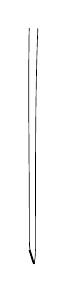
\begin{tikzpicture}[x=1mm,y=1mm,baseline=0pt]
\draw[line width=0.25pt] (0,30) .. controls (-0.15,21) and (0.05,11) .. (0.02,3) .. controls (0.02,1.7) and (0.28,0.8) .. (0.62,0.05);
\draw[line width=0.23pt] (1.1,30) .. controls (0.73,21) and (0.82,10) .. (0.78,2.3) .. controls (0.84,1) and (0.68,0.45) .. (0.62,0.05);
\draw[line width=0.65pt] (0.04,1.8) .. controls (0.25,1.25) and (0.42,0.5) .. (0.62,0.05);
\end{tikzpicture}}
Je présume que (dans la situation actuelle --- ou même, avec un corps de base $K$) on a $N_{x'}=\operatorname{Norm}_{\mathcal E_L}(I_{x'})$, \inserted{(a priori, on a seulement $\subset$)} ce qui est lié à l'idée qu'on doit avoir $I_{x'}=\operatorname{Norm}_{\unsure{\Pi|\pi}_{L/K}}(I_{x'})$

\margin{118}

\scanpage{120}
--- à tirer au clair à l'occasion !

Revenant au modèle $U$, fournissant
un quotient $\mathcal E_U^{\overline L}$ de $\mathcal E_L^{\overline L}$, d'où
$N_{x'}\longrightarrow\mathcal E_U^{\overline L}$, induisant $I_{x'}\longrightarrow\mathcal E_U^{\overline L}$,
\deleted{Il est clair que \unsure{si}}
qui n'est autre que l'hom \unsure{---} $\mathcal E_{\widetilde U_x}\longrightarrow\mathcal E_U$
associé à $\widetilde U_x\longrightarrow U$. \uline{Si} cet hom
factorise par $\widetilde S_x$, il est immédiat
que l'hom induit $I_{x'}\longrightarrow\mathcal E_U^{\overline L}$ est
nul, puisque \inserted{$I_{x'}$} \deleted{\unsure{c'}}est le noyau de
$\mathcal E_{\widetilde U_x}\Longrightarrow\mathcal E_{\widetilde S_x}$, et $\mathcal E_{\widetilde U_x}\longrightarrow\mathcal E_U$ se factorise par
cet hom.
\margin{i.e. \uline{si} $V$ a un ``centre sur $U$'' i.e. domine un anneau local de $U$\ldots}
[ \uline{A t-on une réciproque ?} regarder ! ]
\margin{Ça devrait être le cas pour $U$ ``élémentaire'' à facteurs pas de \uline{types $(0,0)$ ni $(0,1)$\ldots} \unsure{lié à ceci} \unsure{enfin} à l'existence d'un $K$}

Quand on dispose d'un
modèle \uline{projectif} dont $U$ est un ouvert,
on peut dire (par définition valuative de
la propreté) que $V$ a nécessairement
un centre sur $X$, soit $a$, \deleted{et le centre} \inserted{(\uline{NB} $a$ pas}
néc. de codim.1\ldots) et la condition
envisagée tantôt (assurant que $I_{x'}\longrightarrow
\mathcal E_U^{\overline L}$ est nul) est que $a\in U$.
\margin{119}

\scanpage{122}
correspondent exactement (via $x\longmapsto\underline{O}_{\mathfrak X,x}$) aux jauges dans $L$ qui sont ent. de type fini sur $K$, de corps des fractions $L$ --- i.e. aux $V$ précédents.

Sauf erreur, ces deux types de pts de $\mathfrak X$ (qui épuisent \deleted{tout} si $n=1$,\unsure{)} \inserted{qui est le seul cas, avec $n=0$, où $\mathfrak X$ \unsure{est|soit} un schéma !}) sont les seuls pour lesquels $\underline{O}_{\mathfrak X,x}$ soit noethérien. Cependant, on a

\margin{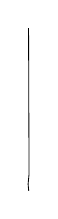
\begin{tikzpicture}[x=1mm,y=\baselineskip]
\draw[line width=0.3pt] (0,0) -- (0.06,-4.4) -- (-0.06,-4.7) -- (0.02,-4.9);
\end{tikzpicture}}
\uline{Proposition} Pour $\forall x\in\mathfrak X$, $\underline{O}_{\mathfrak X,x}$ est un anneau de valuation dans $L$, de corps des fractions $L$, et contenant $K$. L'application $x\longmapsto\underline{O}_{\mathfrak X,x}$ est une bijection de $\mathfrak X$ sur l'ens de ces anneaux dans $L$.
\margin{On pourrait\newline partir d'un\newline schéma excellent\newline $X$, et construire\newline un $\mathfrak X$ relatif au\newline dessus\unsure{\ldots|..}}

\uline{Dém} a) Soit $f\in L\setminus\underline{O}_{\mathfrak X,x}$, il faut prouver $\frac1f\in\underline{O}_{\mathfrak X,x}$. Or $f=g/h$, \inserted{$g,h$}$\in\underline{O}_{X,a}$, où $X$ modèle \inserted{régulier} (propre), $a$ un pt, $f,g$ \deleted{\unsure{premiers} entre eux} --- utilisant la résolution, \deleted{\unsure{on} \uline{\unsure{sépare}} \unsure{les diviseurs}} \inserted{OPS $\exists$ système régulier} de paramètres, avec $f,g$ des monômes
\margin{121}

\scanpage{123}
\mspage{61}

en ces paramètres, et en se ramenant à un $f,g$ premiers entre eux, on est --- faisant encore éclater $a$ --- que les diviseurs de $f,g$ \deleted{\unsure{sont|se}} séparent\ldots

b) Un anneau de val $V$ \deleted{qui} pour l'extension $L/K$ domine un pt bien déterminé \inserted{$x$} de chaque $X$, d'où un $x\in\mathfrak X=\varprojlim X$, et $V$ domine $\underline{O}_{\mathfrak X,x}$, donc lui est égal puisque ce dernier est un anneau de valuation.

\uline{NB} Tout \inserted{modèle $U$ de $\unsure{L|L'}/K$ définit un} \uline{ouvert} de $\mathfrak X$ \deleted{\unsure{correspondant}} \deleted{\unsure{évidemment}} \inserted{(en le plongeant} dans un modèle propre $X$, c'est clair) et \deleted{et} les modèles corres-\\
pondent à \uline{certains} ouverts de $\mathfrak X$ (\uline{pas} \unsure{stables|stable} par réunion finie).

Pour tt anneau loc\textsuperscript{l} \inserted{norm\textsuperscript{l}} $O\subset L$ de corps des fractions $L$, on peut regarder $\operatorname{Spec}\underline{O}=S$, son pt fermé $\unsure{x|s}$, le normali-

\margin{122}

\scanpage{124}
$O'$ de $O$ dans $\overline L$ i.e. $S'$ de $S$ dans $L$, et pour $x'$ au dessus de $x$, un groupe de décomposition $N_{x'}$, d'inertie $I_{x'}$, ayant les interprétations qu'on a signalé plus haut dans le cas particulier d'un $O$ qui est un anneau jauge. L'idée, c'est que prenant $O$ de valuation (pas néc. une jauge) $\supset K$, on trouve des groupes d'inertie à structure simple ---
\margin{$T_\infty=T_\infty(\overline L)$}
des $T_\infty^\alpha$ essentiellement, où $\alpha$ est la ``codim'' du $x\in\mathfrak X$ correspondant --- et si $a$ est de dim $0$, on aur. une extension de $\mathcal E_{k(x)}^{\overline{k(a)}}$ --- ss-groupe ouvert de $\mathcal E_K$, puisque
\margin{on le\newline supposera\newline du moins\newline ici}
$k(a)$ est \inserted{\uline{fini}} alg. sur $K$ --- \deleted{\unsure{de}}\unsure{par} $T^\alpha$, qu'on aura une chance de pouvoir scinder sans trop de mal. Ceci donne-
\margin{123}

\scanpage{125}
\mspage{62}

rait un principe général pour construire des germes de sections de $\mathcal E_L$ sur $\mathcal E_K$ --- à l'aide des pts de dim 0 de la ``variété de Riemann'' $\mathfrak X$ de $L$ sur $K$. Composant, pour une sous-extension $L_1^{\unsure{k|*}}$ de $K$ de degre de tr. 1, avec l'hom $\mathcal E_L\longrightarrow\mathcal E_{L_1}$, on a donc aussi un moyen de construire des \inserted{germes de} sections de $\mathcal E_{L_1}$ sur $\mathcal E_K$, et le fait intéressant sera de voir si on \inserted{en} trouve pas plus que les sections déjà envisagées, associées aux ``places'' de $L_1$ sur $K$.
\margin{on pense ici au cas où $K$ est de type fini sur $\mathbf Q$, bien sûr !}

Mais il en est bien ainsi, comme on voit en considérant $V_1=V\cap L_1$, qui est un anneau de valuation de $L_1$,
\margin{124}

\scanpage{126}
dont le corps résiduel (contenu dans celui de
$V$) sera \deleted{alg} fini sur $K$ si celui de $V$
l'est (donc $V_1\ne L_1$) --- donc $V_1$ \deleted{$\longrightarrow$} \inserted{corresp. \unsure{d} à} une
``place'' du corps de fonctions d'une variable
$L_1$ sur $K$. Or, par des fonctorialités
essentiellement évidentes, on voit que
l'hom $\mathcal E_L^{\overline L}\unsure{\longrightarrow|\twoheadrightarrow}\mathcal E_{L_1}^{\overline{L_1}}$ envoie $N_V$ dans $N_{V_1}$,
$I_V$ dans $I_{V_1}$ --- donc l'image de $N_V$
normalise $I_{V_1}$, donc (si on a une \inserted{germe de} section
de $N_V$ sur $\mathcal E_K$) le germe de section
obtenu de $\mathcal E_{L_1}$ sur $\mathcal E_K$ normalise $I_{V_1}$
--- et sa restriction à $\mathcal E_K^{\unsure{0|\circ}}$ centralise
$I_{V_1}$ ---
\margin{il faut vérifier que le corps des fractions de $V_1$ est bien $L_1$ --- c'est un fait général....}

\uline{Conjecture} Soient $K,L$ des ext. de
type fini de $\mathbf Q$, $K\subset L$. Alors

a) Toute section de $\mathcal E_L$ sur $\mathcal E_K$
(ou germe de tel, ça revient au $=$\ldots)
normalise un $\unsure{I_V|N_V}$ associé à un anneau
de valuation \inserted{$V$} de $L$ contenant $K$, à corps
résiduel algébrique \inserted{sur $K$} \deleted{\unsure{,}} et \deleted{\unsure{ce}} $V$ est uniquement
\margin{125}

\scanpage{127}
\mspage{63}
\margin{À nouveau se pose la question si $N_V=\operatorname{Norm}(I_V)$
On voudrait que les germes de sections de $\mathcal E_L^{\bar L}$, sur \deleted{$\mathcal E_K$} \inserted{$\mathcal E_{K_1}^{\bar K}$} soient associés aux pts du normalisé $\tilde{\mathfrak X}_{L/K}$ de $\mathfrak X_{L/K}$ dans $\bar L$ --- qu'elles forment un fibré sur $\unsure{\tilde{\mathfrak X}|\mathfrak X}_{L/K}$, à fibres les $H^1(\deleted{\mathcal E_K}\inserted{\mathcal E_{K_1}}^{\unsure{G|\bar K}},I_V)\ldots.$
Ceci est associé à la formule (pour une telle section $s$ de $\mathcal E_L$ sur $\mathcal E_K$) $\mathcal E_L^{(\mathcal E_K^{\unsure{0|\circ}})}\simeq I_V$ --- lié à la conjecture que pour tt s-groupe ouvert de $N_V^{\unsure{0|\circ}}$, ou simpl\textsuperscript{t} tt s-groupe de $N_V$ dont l'image dans $N_V/I_V$ soit ouvert, on a \deleted{\unsure{Centr|tout}} $(\mathcal E_L^{\bar L})^{\Gamma}=I_V$ (ceci pour tt anneau de valuation $V$ de $L/K$, \unsure{présumé} de corps rés. alg/$K$)
En fait, la question est purement géométrique \ldots}
\unsure{en|à} cette condition --- en fait la section provient d'une section du groupe de décomposition $N_V$ au dessus de $\mathcal E_K$.

\noindent b) Soit $U$ un modèle ``élémentaire'' de $L$ sur $K$, anabélien. Alors tte section de $\mathcal E_U^{\bar L}$ sur $\mathcal E_K^{\bar K}$ se relève en une section de $\mathcal E_L^{\bar L}$ sur $\mathcal E_K^{\bar K}$.

Elle peut donc se décrire en termes d'un anneau de valuation $V$ de $L/K$, et qd $V$ a un centre sur $U$, \unsure{on n'a qu'à} se concen-\newline trer au cas d'un pt $x\in U$ rationnel sur $K$, et de la section définie par $x$. Dans ce cas (posant tjrs $\Gamma=\mathcal E_K^{\bar K}$) on conjecture encore, bien sûr

\[
(32)\qquad (\mathcal E_L^{\bar L})^{\Gamma^{\unsure{0|\circ}}}=(1)
\]

(et on peut y remplacer $\Gamma^{\unsure{0|\circ}}$ par $\Gamma^{\unsure{0|\circ}}\unsure{\ne1)|\ne)|\subset}\deleted{\unsure{\Gamma}}$
--- mais en fait ceci (en vertu de $\operatorname{Centr}_\Gamma(\Gamma^{\unsure{0|\circ}})=(1)$) équivaut à la relation analogue \deleted{$\unsure{\Pi|\pi}_{L\unsure{/|,}K}^{\bar L}$}

\[
(33)\qquad (\unsure{\Pi|\pi}_{L,K}^{\bar L})^{\Gamma^{\unsure{0|\circ}}}=(1)
\]

qui se déduit d'ailleurs, par dévissage,
\margin{126}

\scanpage{128}
de la conjecture analogue déjà faite pour la dim relative $1$.

Pour mieux appréhender cette deuxi\unsure{è|e}me partie \inserted{b)} de la conjecture, il faudrait examiner de plus près ce que deviennent, par composition avec $\mathcal E_L^{\bar L}\mathrel{\text{---}}\mathcal E_U^{\bar L}$, les sections de $\mathcal E_L^{\bar L}$ sur $\mathcal E_K$ associées à un $V$, et pour commencer, étudier le sous-groupe \inserted{$\Delta_V$} de $\unsure{\pi|\Pi}_{U/K}^{\bar L}$ image de $I_V$ --- qui, on le devine, jouera un rôle analogue à un groupe-bout. Dans quelle mesure des $V$ distinctes definissent-elles des $\Delta_V$ distinctes ?

Pour étudier cette question, introduisons un modèle $X$ de $L/K$ contenant $U$, $X$ propre, les comp. irréd. de \inserted{$D=$} $X-U$ des diviseurs réguliers \inserted{$D_i$ $(i\in I)$}, et $X-U$ à croisements normaux. Pour $x\in\operatorname{supp}D$, considérons le hensélisé \inserted{(pas strict)} $\tilde O_x$ de $\underline{O}_{X,x}$, et l'image inverse $\bar U_x$ de $U$ dessus. On à
\margin{127}

\scanpage{129}
\mspage{64}
$\bar L$ au dessus de $\tilde U_x$, bien sûr, et
\[
 (34)\qquad
 1\mathrel{\text{---}}T^{I(x)}\longrightarrow
 \mathcal E_{\tilde U_x}^{\bar L}\longrightarrow
 \mathcal E_{k(x)}^{\overline{k(x)}}\longrightarrow 1
\]
où \deleted{$I(x)$}
\[
 I(x)=\{i\in I\mid x\in D_i\},\qquad T=T_\infty(\bar L^*)
\]
$\overline{k(x)}$ étant la clôture alg. de $k(x)$ induite par un plongement choisi de $\tilde K_x$ (corps des fonctions de $\widetilde{\underline{O}}_x$) dans $\bar L$, qui fait donc fonction \unsure{égalt|egalt} de clôture sép. de $K_x$.

Ceci dit, pour $V$ anneau de valuation de $L/K$, si son centre $x$ \inserted{sur $X$} est $\in\operatorname{Supp}D$, on aura, pour $S=\operatorname{Spec}V$, d'où $\tilde S$ \inserted{(hensélisé)} du pt générique $\tilde\eta$ une factorisation de $\tilde\eta\longrightarrow U$ (composé $\tilde\eta\longrightarrow\eta=\operatorname{Spec}(L)\longrightarrow U$) en $\tilde\eta\longrightarrow\tilde U_x$, \unsure{car|par} $\tilde\eta\mathrel{\text{---}}U$ est induite par $\tilde S\longrightarrow X$ qui se factorise en $\tilde S\longrightarrow\tilde T\longrightarrow X$ ($\tilde T=\operatorname{Spec}\tilde O_x$). Donc \deleted{l'image $N_V$ de} \inserted{l'hom. induit} $\mathcal E_{\tilde\eta}^{L}\longrightarrow\mathcal E_U^{L}$ est \deleted{contenue dans celle de} \inserted{un composé}
\diagram{\begin{tikzcd}[column sep=large,row sep=0.1em]
 (35) & \mathcal E_{\tilde\eta}^{\bar L}\arrow[r] &
 \mathcal E_{\tilde U_x}^{\bar L}\arrow[r] &
 \mathcal E_U^{\bar L}\\
 & \parallel & \deleted{\unsure{\parallel}}\quad\parallel\ \mathrm{dfn} &\\
 & N_V & \deleted{\unsure{N_x}}\quad N_x &
\end{tikzcd}}
(l'image de $\mathcal E_{\tilde U_x}^{\bar L}\longrightarrow\mathcal E_U^{\bar L}$ n'étant d'ailleurs autre que le groupe de décomposition de $x$ dans $\mathcal E_U^{\bar L}$ relatif à $\bar L$....). L'étude de l'hom composé
\margin{128}
